%
% paper.tex -- Buch zum mathematischen Seminar Variationsprinzipien
%
% (c) 2022 Prof. Dr. Andreas Mueller, OST Ostschweizer Fachhochschule
%
\def\IncludeBookCover{0}
\documentclass{book}
\input{common/packages.tex}

% additional packages used by the individual papers, add a line for
% each paper
\input{papers/common/addpackages.tex}

% PDF info
\hypersetup{
pdftitle={Mathematisches Seminar Variationsprinzipien},
pdfauthor={Andreas Müller}
}

% workaround for biblatex bug
\makeatletter
\def\blx@maxline{77}
\makeatother
\addbibresource{../chapters/references.bib}

% Bibresources for each article
\input{papers/common/addbibresources.tex}

%\pgfplotsset{compat=1.12}
\setlength{\headheight}{15pt} % fix headheight warning
\DeclareGraphicsRule{*}{mps}{*}{}
\begin{document}

%
% macros.tex -- some common macro definitions
%
% (c) 2021 Prof Dr Andreas Müller, OST Ostschweizer Fachhochschule
%
\hypersetup{
    linktoc=all,
    linkcolor=blue
}
\newcounter{beispiel}
\newenvironment{beispiele}{
\bgroup\smallskip\parindent0pt\bf Beispiele\egroup

\begin{list}{\arabic{beispiel}.}
  {\usecounter{beispiel}
  \setlength{\labelsep}{5mm}
  \setlength{\rightmargin}{0pt}
}}{\end{list}}
\newcounter{uebungsaufgabezaehler}
% environment fuer uebungsaufgaben
\newenvironment{uebungsaufgaben}{%
}{%
\vfill\pagebreak}
\newenvironment{teilaufgaben}{
\begin{enumerate}
\renewcommand{\theenumi}{\alph{enumi})}
%\renewcommand{\labelenumi}{\alph{enumi})}
\renewcommand{\labelenumi}{\theenumi}
}{\end{enumerate}}
% Aufgabe
\newcounter{problemcounter}[chapter]
\def\aufgabenpath{chapters/uebungsaufgaben/}
\def\ainput#1{\input\aufgabenpath/#1}
\def\verbatimainput#1{\expandafter\verbatiminput{\aufgabenpath/#1}}
\def\aufgabetoplevel#1{%
\expandafter\def\expandafter\inputpath{#1}%
\let\aufgabepath=\inputpath
}
\def\includeagraphics[#1]#2{\expandafter\includegraphics[#1]{\aufgabepath#2}}
% \aufgabe
\renewcommand\theproblemcounter{\thechapter.\arabic{problemcounter}}
\newcommand{\uebungsaufgabe}[1]{%
\refstepcounter{problemcounter}%
\label{#1}%
\bigskip{\parindent0pt\strut}\hbox{\bf\theproblemcounter. }%
\expandafter\def\csname aufgabenpath\endcsname{\inputpath/}%
\expandafter\input{\aufgabenpath/#1.tex}
}
% linsys
\newcolumntype{\linsysR}{>{$}r<{$}}
\newcolumntype{\linsysL}{>{$}l<{$}}
\newcolumntype{\linsysC}{>{$}c<{$}}
\newenvironment{linsys}[1]{%
\begin{tabular}{*{#1}{\linsysR@{\;}\linsysC}@{\;}\linsysR}}%
{\end{tabular}}

% Loesung
\def\swallow#1{
%nothing
}
\NewEnviron{loesung}[1][Lösung]{%
\begin{proof}[#1]%
\renewcommand{\qedsymbol}{$\bigcirc$}
\BODY
\end{proof}
}
\NewEnviron{bewertung}{%
\begin{proof}[Bewertung]%
\renewcommand{\qedsymbol}{}
\BODY
\end{proof}
}
\NewEnviron{diskussion}{%
\begin{proof}[Diskussion]%
\renewcommand{\qedsymbol}{}
\BODY
\end{proof}
}
\NewEnviron{hinweis}{%
\begin{proof}[Hinweis]%
\renewcommand{\qedsymbol}{}
\BODY
\end{proof}
}
\def\keineloesungen{%
\RenewEnviron{loesung}{\relax}
\RenewEnviron{bewertung}{\relax}
\RenewEnviron{diskussion}{\relax}
}
\newenvironment{beispiel}{%
\refstepcounter{satz}
\begin{proof}[Beispiel \arabic{chapter}.\arabic{satz}]%
\renewcommand{\qedsymbol}{$\bigcirc$}
}{\end{proof}}

\allowdisplaybreaks

\lhead{Inhaltsverzeichnis}
\rhead{}
\tableofcontents
\newtheorem{satz}{Satz}[chapter]
\newtheorem{hilfssatz}[satz]{Hilfssatz}
\newtheorem{korollar}[satz]{Korollar}
\newtheorem{lemma}[satz]{Lemma}
\newtheorem{definition}[satz]{Definition}
\newtheorem{annahme}[satz]{Annahme}
\newtheorem{frage}[satz]{Frage}
\newtheorem{problem}[satz]{Problem}
\newtheorem{aufgabe}[satz]{Aufgabe}
\newtheorem{prinzip}[satz]{Prinzip}
\newtheorem*{problem*}{Problem}
\newtheorem{forderung}{Forderung}[chapter]
\newtheorem{konsequenz}[satz]{Konsequenz}
\newtheorem{algorithmus}[satz]{Algorithmus}

% English variants
\newtheorem{theorem}[satz]{Theorem}

\renewcommand{\floatpagefraction}{0.7}

\definecolor{darkgreen}{rgb}{0,0.6,0}
\definecolor{darkred}{rgb}{0.8,0,0}
\definecolor{orange}{rgb}{1,0.6,0}
\definecolor{gelb}{rgb}{1,0.8,0}
%
% Kopfzeilen
%
\fancyfoot{}
\fancyhead{}
%\def\kopfrechts#1{
%\edef\theshortsection{\arabic{section}}
%\rhead{\theshortsection. #1}}
%\def\kopflinks#1{\lhead{\thechapter. #1}
%\rhead{}}
\def\kopfrechts#1{
\global\def\kopfinhalt{#1}
\xdef\theshortsection{\thechapter.\arabic{section}}
\fancyhead[LO]{\theshortsection. #1}}
%
\def\kopflinks#1{
\global\def\kapitelinhalt{#1}
\fancyhead[RE]{\thechapter. #1}
\thispagestyle{empty}
\fancyhead[LO]{}}
%
%
% Uebungsaufgaben
%
\def\uebungsabschnitt{%
\begingroup

\bigskip

\noindent
\vbox to0.3cm{\hbox to\textwidth{\normalfont\large\bfseries Übungsaufgaben}\vfill}
%\keineloesungen%
\nopagebreak%
\fancyhead[RE]{\thechapter. \kapitelinhalt}%
\fancyhead[LE]{\thepage}%
\fancyhead[LO]{Übungsaufgaben}%
\fancyhead[RO]{\thepage}%
\addcontentsline{toc}{section}{Übungsaufgaben}%
}
\def\enduebungsabschnitt{
\endgroup
\bigskip
}
%
\fancyhead[LE]{\thepage}
\fancyhead[RO]{\thepage}
% Transposition
\def\transpose#1{{{#1}^t}}
% Real- und Imaginaerteil
\def\Re{\operatorname{Re}}
\def\Im{\operatorname{Im}}
\def\tr{\operatorname{tr}}
\def\sign{\operatorname{sign}}
\def\grad{\operatorname{grad}}
\def\supp{\operatorname{supp}}%
%
% Gauss-Operations from LinAlg-Book
% macros for gauss operations, they all have 4 arguments
%
% #1  width (cm)
% #2  height (cm)
% #3  offset-x (units required)
% #4  offset-y (units required)
%
\def\pivotoperationr{0.2}
% a rounded rectangle around the pivot element
\def\pivotoperation#1#2#3#4{
\smash{\rlap{\raisebox{#4}{\hspace{#3}\begin{tikzpicture}[thick]
\def\p{
	({#1/2},0)
	-- +(0,{(#2/2)-\pivotoperationr}) arc (0:90:\pivotoperationr)
	-- +({-(#1)+2*\pivotoperationr},0) arc (90:180:\pivotoperationr)
	-- +(0,{-(#2)+2*\pivotoperationr}) arc(180:270:\pivotoperationr)
	-- +({#1-2*\pivotoperationr},0) arc(270:360:\pivotoperationr) 
	-- cycle
}
\fill[color=red!20] \p;
\draw[color=red] \p;
\end{tikzpicture}}}}}
% a circle around the pivot element
\def\pivotoperationcircle#1#2#3{
\smash{\rlap{\raisebox{#3}{\hspace{#2}\begin{tikzpicture}[thick]
\def\p{ ({#1/2},0) arc (0:360:{#1/2}) -- cycle
}
\fill[color=red!20] \p;
\draw[color=red] \p;
\end{tikzpicture}}}}}
% forwardreduction
\def\forwardreduction#1#2#3#4{
\smash{\rlap{\hspace*{#3}\raisebox{#4}{\begin{tikzpicture}[thick]
\def\p{
	(#1,-0.25)
	-- +(0,{#2-\pivotoperationr}) arc(0:90:\pivotoperationr)
	-- +({-#1+2*\pivotoperationr},0) arc (90:180:\pivotoperationr)
	-- +(0,{-#2+\pivotoperationr)})
}
\fill[color=blue!20] \p -- cycle;
\draw[color=blue] \p;
\end{tikzpicture}}}}
}
% backwardsubstitution
\def\backwardsubstitution#1#2#3#4{
\smash{\rlap{\hspace*{#3}\raisebox{#4}{\begin{tikzpicture}[thick]
\def\p{
	({#1},0.25)
	-- +(0,{-#2+\pivotoperationr}) arc(0:-90:\pivotoperationr)
	-- +({-#1+2*\pivotoperationr},0) arc(-90:-180:\pivotoperationr)
	-- +(0,{#2-\pivotoperationr})
}
\fill[color=blue!20] \p -- cycle;
\draw[color=blue] \p;
\end{tikzpicture}}}}
}
% zerorow
\def\zerorow#1#2#3#4{
\smash{\rlap{\hspace*{#3}\raisebox{#4}{\begin{tikzpicture}[thick]
\def\p{ (0,0) rectangle (#1,#2) }
\fill[color=orange!20] \p -- cycle;
%\draw[color=blue] \p;
\end{tikzpicture}}}}
}


\mainmatter

%
% main.tex -- Paper zum Thema <schwimmen>
%
% (c) 2020 Autor, OST Ostschweizer Fachhochschule
%
% !TEX root = ../../buch.tex
% !TEX encoding = UTF-8
%

\chapter{Die Optimale Flussüberquerung\label{chapter:schwimmen}}
\kopflinks{Die optimale Flussüberquerung}
\begin{refsection}
\chapterauthor{Anna Pietak}


Das Überqueren eines Flusses ist seit jeher eine Herausforderung, die die Menschheit beschäftigt. Oft auch im Zusammenhang mit der Frage, wie man am besten mit einem Boot einen Fluss überquert, sind vielfältige Überlegungen angestellt worden. So hat sich auch Euler in seinem Werk \textit{De motu cymbarum remis propulsarum in fluviis} \cite{schwimmen:Euler_works} diese Frage gestellt. Einige einfache Ansätze könnten darin bestehen, den Fluss an einer flachen Stelle zu überqueren, wo man zu Fuss hindurch waten kann, oder ihn einfach gemütlich schwimmend zu durchqueren und einfach in kauf nehmen, dass die Strömung einen mitreisst.
	
	
Die zentrale Frage, die sich hier stellt, ist jedoch: Wie überquere ich einen Fluss am energieeffizientesten? In Abbildung \ref{fig:river_original} ist ein solcher Fluss dargestellt, der überquert werden soll.

%
% fig-fluss.tex -- Darstellung des Flusses
%
% (c) 2024 Anna Pietak
%
\begin{figure}
    \centering
    \tikzset{every picture/.style={line width=0.75pt}} %set default line width to 0.75pt        

    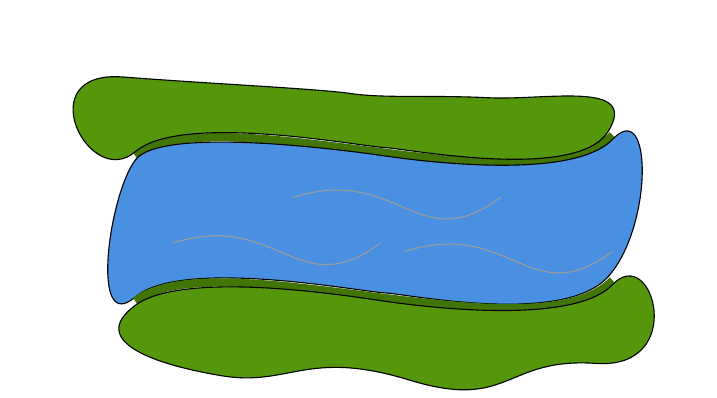
\begin{tikzpicture}[x=0.75pt,y=0.75pt,yscale=-1,xscale=1]
%uncomment if require: \path (0,300); %set diagram left start at 0, and has height of 300

%Curve Lines [id:da608977851192717] 
\draw [color={rgb, 255:red, 65; green, 117; blue, 5 }  ,draw opacity=1 ][line width=3]    (300,110) .. controls (340,80) and (493.51,138.06) .. (530,100) ;
%Shape: Polygon Curved [id:ds9392726871646548] 
\draw  [fill={rgb, 255:red, 74; green, 144; blue, 226 }  ,fill opacity=1 ] (300,112) .. controls (312.68,95.2) and (403.92,107.66) .. (420,110) .. controls (436.08,112.34) and (510.65,122.34) .. (530,102) .. controls (549.35,81.66) and (549.3,143.91) .. (528,168) .. controls (506.7,192.09) and (432.13,176.66) .. (420,176) .. controls (407.87,175.34) and (322.13,158.94) .. (300,178) .. controls (277.87,197.06) and (287.32,128.8) .. (300,112) -- cycle ;
%Curve Lines [id:da6433547723995421] 
\draw [color={rgb, 255:red, 65; green, 117; blue, 5 }  ,draw opacity=1 ][line width=3]    (300,180) .. controls (340,150) and (493.51,208.06) .. (530,170) ;
%Shape: Polygon Curved [id:ds34371397326569686] 
\draw  [fill={rgb, 255:red, 85; green, 151; blue, 11 }  ,fill opacity=1 ] (300,182) .. controls (323.56,164.66) and (403.92,177.66) .. (420,180) .. controls (436.08,182.34) and (510.65,192.34) .. (530,172) .. controls (549.35,151.66) and (566.44,213.06) .. (522,210) .. controls (477.56,206.94) and (481.01,233.06) .. (432,218) .. controls (382.99,202.94) and (374.13,221.23) .. (342,216) .. controls (309.87,210.77) and (276.44,199.34) .. (300,182) -- cycle ;
%Shape: Polygon Curved [id:ds3342416894164969] 
\draw  [fill={rgb, 255:red, 85; green, 151; blue, 11 }  ,fill opacity=1 ] (294,72) .. controls (339.58,75.49) and (387.92,77.66) .. (404,80) .. controls (420.08,82.34) and (442.15,80.63) .. (470,82) .. controls (497.85,83.37) and (542.72,73.49) .. (528,98) .. controls (513.28,122.51) and (432.13,106.66) .. (420,106) .. controls (407.87,105.34) and (322.13,88.94) .. (300,108) .. controls (277.87,127.06) and (248.42,68.51) .. (294,72) -- cycle ;
%Curve Lines [id:da7504908272245701] 
\draw [color={rgb, 255:red, 155; green, 155; blue, 155 }  ,draw opacity=1 ]   (318,152) .. controls (369.01,135.91) and (378,182) .. (418,152) ;
%Curve Lines [id:da01966435364089625] 
\draw [color={rgb, 255:red, 155; green, 155; blue, 155 }  ,draw opacity=1 ]   (376,130) .. controls (427.01,113.91) and (436,160) .. (476,130) ;
%Curve Lines [id:da5498107083025197] 
\draw [color={rgb, 255:red, 155; green, 155; blue, 155 }  ,draw opacity=1 ]   (430,156) .. controls (481.01,139.91) and (490,186) .. (530,156) ;




\end{tikzpicture}

    \caption{Fluss der überquert werden soll. Blau ist der Fluss eingezeichnet und grün das Ufer.}
    \label{fig:river_original}
\end{figure}
%

Für die Frage \textit{Wie schwimmt man am besten durch den Fluss?} wird zudem vorausgesetzt, dass das Ziel auf derselben Höhe auf der anderen Seite des Flusses erreicht werden soll. Was bedeutet das man die ganze Strömung durch flussaufwärs schwimmen kompensiert werden muss. Dies ist in Abbildung \ref{fig:river_points} veranschaulicht. Die Frage, die uns hier beschäftigt, lautet: Wie schwimmt man am besten von Punkt \(A\) nach Punkt \(B\)?

\input{papers/schwimmen/fig-ueberquerung.tex}%

In diesem Kapitel wird erläutert, wie man mittels des Variationsprinzips die optimale Schwimmroute über den Fluss findet, sodass man den geringsten Energieaufwand hat.


%
% o1_herangehensweise.tex -- Beispiel-File für die Einleitung
%
% (c) 2020 Prof Dr Andreas Müller, Hochschule Rapperswil
%
% !TEX root = ../../buch.tex
% !TEX encoding = UTF-8
%
\section{Herangehensweise\label{schwimmen:section:teil0}}
\kopfrechts{Herangehensweise}

Es soll ermittelt werden, welche die energieeffizienteste Methode
ist, um den Fluss zu überqueren. Da die Energie \(E\) mittels der
Formel \[E = P \cdot t\] berechnet werden kann, wobei \(P\) für die
Leistung und \(t\) für die Zeit steht, stellt sich heraus, dass die
Energie für die Flussüberquerung direkt von der Zeit abhängt. Ergo
sollte es möglich sein, nicht die Energie zu optimieren, sondern
die Zeit.

Dies vereinfacht vieles, allerdings muss nun die Leistung, mit der
geschwommen werden kann, begrenzt werden. Eine schwimmende Person
kann nicht unbegrenzt schnell schwimmen und somit nicht in beliebig
kurzer Zeit am anderen Ufer ankommen.

\subsection{Variationsprinzip}
Das Variationsprinzip ist ein Konzept, das besagt, dass die Natur
in vielen Fällen den optimalen Weg wählt. In diesem Fall ist es das
Prinzip der kleinsten Wirkung, also des kleinsten Energieaufwand,
der für die Flussüberquerung benötigt wird. Die
Euler-Lagrange-Differentialgleichung ist das Werkzeug, um das
Variationsprinzip zu berechnen. Das Integral der Lagrange-Funktion
gibt das Minimum der Wirkung zurück.



%
% teil1.tex -- Beispiel-File für das Paper
%
% (c) 2020 Prof Dr Andreas Müller, Hochschule Rapperswil
%
% !TEX root = ../../buch.tex
% !TEX encoding = UTF-8
%
\section{Herleitung
\label{schwimmen:section:naiver_weg}}
\kopfrechts{Problemstellung}

Hier ist eine Schritt für Schritt Darstellung der Herleitung zur optimalen Flussüberquerung dargestellt. Als inspiration der Bilder und der Herangehensweise wurde an die Forumsfrage in \cite{schwimmen:mathForum} angelehnt. 

% papers/schwimmen/
\begin{figure}
    \centering
        \centering
        \includegraphics[width=0.6\textwidth]{papers/schwimmen/Grafiken/Figure_1-crop.png}	
        \caption{Fluss mit quadratischer Strömung. Ziel ist es von Punkt \((0,0)\) zum Punkt \((a,A)\) zu kommen, der auf der anderen Uferseite, auf gleicher Höhe, liegt.}
        \label{fig:river_template}
\end{figure}

Ziel ist es die schnellste Rute über den Fluss zu finden. In Abbildung \ref{fig:river_template} ist dies abgebildet, wobei \(a\) die Flussbreite ist und \(A\) die Distanz entlang des Flusses. Im Falle unserer Aufgabenstellung ist \(A=0\) da man am andern Ufer auf gleicher Höhe ankommt.

\subsubsection{Wichtige Kenngrössen}
Ein paar wichtige Kenngrössen für die Herleitung sind in Tabelle \ref{table:Wichtige_Kenngroessen} zufinden.

\begin{table}
    \centering
    \renewcommand{\arraystretch}{1.3}
    \begin{tabularx}{\textwidth}{@{}ll>{\raggedright\arraybackslash}p{7cm}@{}}
        \multicolumn{3}{c}{Wichtige Grössen} \\
        % \specialrule{.1em}{.05em}{.05em}
        % \textbf{Dataset} & \textbf{\(\mu\) in \(\mathrm{ps}\)} & \textbf{\(\sigma\) in \(\mathrm{ps}\)} \\
        \hline
        \(a\)   &   Flussbreite  &   definiert von der Umgebung \\
        \(c\)   &   Schwimmgeschwindigkeit        &   Definiert von der schwimmenden Person       \\
        \(v(x)\)   &   Flussgeschwindigkeit         &   Ist von der \(x\)-Position im Fluss abhängig     \\
        \((0,0)\)   &   Startpunkt         &   Startpunkt am Flussufer     \\
        \((a,A)\)   &   Endpunkt         &   Endpunkt auf anderer Uferseite aber auf gleicher Höhe     \\
        \specialrule{.1em}{.05em}{.05em}
    \end{tabularx}
    \caption{Wichtige Kenngrössen für die Herleitung}
    \label{table:Wichtige_Kenngroessen}
\end{table}


\subsubsection{Schwimmgeschwindigkeiten}

Als erstes werden die Geschwindigkeiten der schwimmenden Person definiert. Mittels den Schwimmrichtungsvektoren und dem Flussvektor können folgende Geschwindigkeiten für die in \(x\)- und \(y\)-Richtungen geschwommenen Geschwindigkeiten relativ zum Ufer genommen werden:
\begin{align}
    c_x &= c\cdot \cos(\theta) \label{eq:c_x_equation}\\
    c_y &= u(x) + c \cdot \sin(\theta) \label{eq:c_y_equation}
\end{align}
\(c_x\) ist die Geschwindigkeit in \(x\)-Richtung der schwimmenden Person, \(c_y\) ist die Geschwindigkeit in \(y\)-Richtung wie auch die Flussgeschwindigkeit. Dabei ist der Winkel \(\theta\) der Schwimmwinkel in Bezug auf die \(x\)-Richtung.


\subsubsection{Zeitoptimierung}

Da für den geringsten Energiekonsum die Zeit optimiert wird, hier das Integral für die total gebrauchte Zeit der Flussüberquerung:
\begin{equation}
    T = \int_0^adt \label{eq:Time_river_1}
\end{equation}
Da \(dt = \frac{dx}{c_x}\), die Zeit die es benötigt um sich ein kleines Stück in \(x\)-Richtung zu bewegen, von der Geschwindigkeit in \(x\)-Richtung abhängt, kann man \eqref{eq:Time_river_1} erweitern zu

\begin{equation}
    T = \int_0^adt = \int_0^a\frac{dx}{||c_x||} = \int_0^a\frac{dx}{c\cdot \cos(\theta)} \label{eq:Time_river_2},
\end{equation}
wobei \(||c_x||\) den Vektor \(c_x\) definiert. 


\subsubsection{Beziehung der \(x\)- und \(y\)-Geschwindigkeiten}

Als nächstes die Beziehung der \(x\)- und \(y\)-Geschwindigkeiten im System behandelt. Dies ist auch am Schluss wichtig um den genauen Schwimmverlauf der schwimmenden Person beobachten zu können.

Die \(y\)-Geschwindigkeit soll im Bezug zur \(x\)-Richtung gegeben werden. Die Schwimmgeschwindigkeit in \(y\)-Richtung is gegeben durch
\begin{equation}
    c_y = \frac{dy}{dt}
\end{equation}
worauf die Kettenregel angewendet werden kann um
\begin{equation}
    \frac{dy}{dt} = \frac{dy}{dx} \cdot \frac{dx}{dt} = \frac{dy}{dx}\cdot c_x = \frac{dy}{dx}\cdot c\cdot \cos(\theta)
\end{equation}
zubekommen. Mittels \(c_y = u(x) + c\cdot \sin(\theta)\) bekommt man die Beziehung der \(x\)- und \(y\)-Geschwindigkeiten:
\begin{equation}
    \frac{dy}{dx} = \frac{u(x) + c \cdot \sin(\theta)}{c \cdot \sin(\theta)} \label{eq:dy_dx}
\end{equation}



\subsubsection{Auflösen nach \(\theta\)}

Der letzte Schritt für das aufstellen des Integrals ist es eine Formel für den Winkel \(\theta\) zu haben.
Ausgehend von \eqref{eq:dy_dx} können Umformungen gemacht werden
\begin{align}
    \frac{dy}{dx} &= \frac{\dot{y}}{\dot{x}} = \frac{c_y}{c_x} = \frac{u(x) + c \cdot \sin(\theta)}{c \cdot \sin(\theta)} \\
    \frac{dy}{dx} &= \frac{u}{c}\cdot \sec(\theta) + \tan(\theta) \\
    \frac{dy}{dx} &= \frac{u}{c}\cdot \sec(\theta) + \sqrt{\sec^2(\theta)-1}. \\
\end{align}

Es sind folgende Formeln für die Umformungen zu beachten: \[\frac{1}{\cos(\theta)} = \sec(\theta)\] und \[\sec^2(\theta)-\tan^2(\theta) = 1.\] Durch Quardrieren und \[\frac{dy}{dx} = y'\] folgt 
\begin{equation}
    \biggl(\frac{u^2}{c^2}-1 \biggr) \cdot \sec^2(\theta) - \frac{2uy'}{c}\cdot \sec(\theta) + y'^2 +1 = 0
\end{equation}
als Gleichung. Durch die Mitternachtsformel bekommt man 
\begin{equation}
    \sec(\theta) = \frac{\frac{2uy'}{c} \pm \sqrt{4(y'^2-\frac{u^2}{c^2} + 1)}}{2(\frac{u^2}{c^2}-1)}
\end{equation}
für den Winkel \(\theta\). Durch weiteres Umformen bekommt man:
\begin{equation}
    \frac{1}{c}\cdot \sec(\theta) = \frac{-uy' \mp \sqrt{c^2(y'^2+1)-u^2}}{c^2-u^2} .\label{eq:theta_1}
\end{equation}


\subsubsection{Zeit Integral}

Nun kann man die Formel \eqref{eq:theta_1} für den Winkel, in das Zeit-Integral einfügen:

\begin{equation}
    T = \int_0^adt = \int_0^a\frac{dx}{c\cdot \cos(\theta)} = \int_0^a \frac{-uy' \mp \sqrt{c^2(y'^2+1)-u^2}}{c^2-u^2} dx
    \label{eq:Time_river_2} 
\end{equation}
Dieses Integral  beschreibt die Zeit die für die Flussüberquerung benötigt wird. 



\subsubsection{Lagrange-Funktion} 
Um die Rute zu finden, die die kürzeste Zeit für die Flussüberquerung benötigt wendet man das Variationsprinzip. Für das braucht man die sogenannte Funktional welches minimiert werden soll in diesem Fall \eqref{eq:Time_river_2}. 
Aus dem Funktional \eqref{eq:Time_river_2} kann die Lagrange-Funktion
\begin{equation}\label{eq:lagrange_integral}
    L(x, y, y') = \frac{-uy' \mp \sqrt{c^2(y'^2+1)-u^2}}{c^2-u^2}
\end{equation}
herausgelesen werden. 

\subsubsection{Euler-Lagrange-Differentialgleichung} Die Euler-Lagrange-Differentialgleichung kann vereinfacht werden, da sie nicht direkt von \(y\) abhängig ist:

\begin{align}
    \frac{\partial L}{\partial y} - \frac{d}{dx}\frac{\partial L}{\partial y'} = 0 - \frac{d}{dx}\frac{\partial L}{\partial y'} &= 0 \\
    \frac{d}{dx}\frac{\partial L}{\partial y'} &= 0.
\end{align}
Daraus folgt die Ableitung der Lagrange-Funktion:
\begin{align}
    \frac{\partial L}{\partial y'} &= \text{constant} \label{eq:Lagrange_derivites_1}\\
    \frac{\partial L}{\partial y'} &= \frac{\partial}{\partial y'} \biggl (\frac{-uy' \mp \sqrt{c^2(y'^2+1)-u^2}}{c^2-u^2}\biggr) \\
    &= \frac{c^2\cdot y'}{\sqrt{c^2(y'^2-u^2)}(c^2-u^2)} - \frac{u}{c^2-u^2} \\
    &=  \frac{1}{c^2-u^2} \biggl( \frac{c^2\cdot y'}{\sqrt{c^2(y'^2-u^2)}} - u \biggr ) \\
    &= \text{constant} = \frac{1}{g}.\label{eq:Lagrange_derivites_2}
\end{align}
Auflösung nach \(y'\) ergiebt
   
\begin{equation}
    y' = \frac{c^2 + g\cdot u - u^2}{c \cdot \sqrt{u^2-2\cdot g\cdot u - c^2 + g^2}} .\label{eq:angle} \\
\end{equation}
\(y'\) gibt an mit welchem Verhältnis von \(y\) zu \(x\) sich die Schwimmende Person im Wasser bewegt.
































% \subsubsection{Zeitoptimierung} Die Zeit \(T\), die für die Flussüberquerung benötigt wird, kann mittels
% \[
% T = \int \frac{1}{v} \, ds
% \]
% berechnet werden, wobei \(v\) die Geschwindigkeit ist und \(s\) die dabei zurückgelegte Strecke.

% \subsubsection{Zeit für ein Streckenstück} Die Zeit, die für ein sehr kleines Streckenstück entlang der Schwimmroute benötigt wird, kann ermittelt werden, indem man diese kleine Strecke durch die Geschwindigkeit auf dieser kleinen Strecke teilt. Dies sieht so aus:
% \begin{equation}\label{eq:time_for_distance_pice}
%     \frac{ds}{\sqrt{(c_y - u)^2 + c_x^2}},
% \end{equation}
% wobei \(u\) die Geschwindigkeit des Flusses bzw. der Strömung an dieser Stelle im Fluss ist. \(c_x\) und \(c_y\) bezeichnen die Geschwindigkeiten der schwimmenden Person in \(x\)- und \(y\)-Richtung, relativ zum Ufer. Die korrektur mit \(u\) dient der Kompenation der Strömung. Eine grafische Darstellung ist in Abbildung \ref{fig:river_dif} zu sehen.

% \subsubsection{Zeit für die Strömungskompensation} Die Zeit, die zusätzlich zur Flussüberquerung benötigt wird, um die Strömung zu kompensieren, ist definiert als 
% \begin{equation}\label{eq:time_compenation}
%     \frac{dx}{u}.
% \end{equation}

% \subsubsection{Gesamte Zeit} Die gesamte Zeit für ein sehr kleines Streckenstück kann mittels der Gleichungen \eqref{eq:time_for_distance_pice} und \eqref{eq:time_compenation} hergeleitet werden. Es folgt für die Zeit eines Wagestücks
% \begin{equation}\label{eq:time_pice_total}
%     dt = \frac{dx}{u} + \frac{ds}{\sqrt{(c_y - u)^2 + c_x^2}}.
% \end{equation}

% \subsubsection{Strecke}
% Für allgemeine Fälle kann die Distanz einer Strecke mit der Formel
% \[
% ds = \sqrt{\Delta x^2 + \Delta y^2} \approx \sqrt{1 + y'^2} \, dx
% \]
% angenähert werden, wobei sich die Variablen wieder auf Abbildung \ref{fig:river_dif} beziehen.

% \subsubsection{Integral} Nun ist es an der Zeit, ein Integral für die Zeit, die benötigt wird, um den Fluss zu überqueren, aufzustellen, basierend auf den obigen Formeln. Das Integral wird entlang \(x\), also vom einten Ufer \(A\) zum anderen Ufer \(B\), des Flusses, entlang Integriert. Das Integral
% \begin{equation}\label{eq:integral_time}
%     T = \int_A^B L(x, y, y') \, dx = \int_A^B \biggl( \frac{1}{u} + \frac{\sqrt{1 + y'^2}}{\sqrt{(c_y - u)^2 + c_x^2}} \biggr) dx
% \end{equation}
% soll für eine möglichst kleine Zeit \(T\) optimiert werden, um die energieeffizienteste Überquerung zu erreichen. Es ist zu beachten das \(u\), \(c_x\), \(c_y\) sowohl als auch \(y'\) von x abhängig sind, bzw. sie sind alle von der aktuellen Position im Fluss abhängig. Somit müssten sie eigentlich \(u(x)\), \(c_x(x)\), \(c_y(x)\) sowohl als auch \(y'(x)\) heisen, der Einfachheitshalber werden sie aber nur in der verkürzten Schreibweise geschrieben.

% \subsubsection{Lagrange-Funktion} Aus dem Lagrange-Integral \ref{eq:integral_time} kann die Lagrange-Funktion
% \begin{equation}\label{eq:lagrange_integral}
%     L(x, y, y') = \frac{1}{u} + \frac{\sqrt{1 + y'^2}}{\sqrt{(c_y - u)^2 + c_x^2}}
% \end{equation}
% herausgelesen werden. Die Lagrange-Funktion wird für das Variationsprinzip benötigt, um die Funktion für die energieeffizienteste Methode für die Flussüberquerung zu berechnen. Wobei \(y'\) angibt wie schnell sich die schwimmende Person in y-Richtung bewegt während sie sich in x-Richtung bewegt.

% \subsubsection{Euler-Lagrange-Differentialgleichung} Die Euler-Lagrange-Differentialgleichung kann vereinfacht werden, da sie nicht direkt von \(y\) abhängig ist:

% \begin{align}
%     \frac{\partial L}{\partial y} - \frac{d}{dx}\frac{\partial L}{\partial y'} = 0 - \frac{d}{dx}\frac{\partial L}{\partial y'} &= 0 \\
%     \frac{d}{dx}\frac{\partial L}{\partial y'} &= 0.
% \end{align}

% Daraus folgt die Ableitung der Lagrange-Funktion:
% \begin{align}
%     \frac{\partial L}{\partial y'} &= \text{constant} \label{eq:Lagrange_derivites_1}\\
%     \frac{\partial L}{\partial y'} &= \frac{\partial}{\partial y'} \biggl( \frac{1}{u} + \frac{\sqrt{1 + y'^2}}{\sqrt{(c_y - u)^2 + c_x^2}} \biggr) \\
%     &= \frac{1}{\sqrt{(c_y - u)^2 + c_x^2}} \cdot \frac{y'}{\sqrt{1 + y'^2}}\\
%     &= \text{constant} = \frac{1}{g}.\label{eq:Lagrange_derivites_2}
% \end{align}
% Auflösung nach \(y'\):
% \begin{align}
%     y' &= \sqrt{(c_y - u)^2 + c_x^2} \cdot \sqrt{1 + y'^2} \cdot \frac{1}{g} \\
%     y' &= \sqrt{\frac{c_y^2 - 2 \cdot c_y \cdot u + u^2 + c_x^2}{g^2 - c_y^2 + 2 \cdot c_y \cdot u - u^2 - c_x^2}}.\label{eq:angle}
% \end{align}

% \(y'\) gibt an wie schnell sich die schwimmende Person in y-Richtung während sie sich in x-Richtung bewegt, um das andere Ufer am Effizientesten zu erreichen.


% Wird das Integral über \(y'\) gebildet, erhält man die Zeit:
% \begin{equation}\label{eq:time_integral}
%     T = y = \int \sqrt{\frac{c_y^2 - 2 \cdot c_y \cdot u + u^2 + c_x^2}{g^2 - c_y^2 + 2 \cdot c_y \cdot u - u^2 - c_x^2}} \, dx
% \end{equation}





















        

%     \caption{Fluss der überquert werden soll. Die Strömungsgeschwindigkeit \(u\) dunkelblau eingezeichnet beziht sich auf die geschwindigkeit des Flusses, dabei ist zu beachten das diese nicht überal im Fluss gleich sein muss, sie könnte zum Ufer des Flusses hin langamer sein und in der mitte des Flusses schneller. Somit ist sie von \(x\) abhängig. \(c_x\)} und \(c_y\) bezeichenen die Geschwindigkeiten in \(x\)- und \(y\)-Richtung der schwimmenden Person. \(\Delta x\) und \(\Delta y\) sind die sehr kleinen Distanzen auf der Strecke von A nach B.
%     \label{fig:river_dif}
% \end{figure}


% \textbf{Zeitoptimierung} Die Zeit \(T\) die Für die Flussüberquerung gebraucht wird kann mittels \[T=\int{\frac{1}{v}ds}\] berechnet werden, wobei \(v\) die Geschwindigkeit ist und \(s\) die dabei zurückgelegte Strecke. 

% \textbf{Zeit für ein Streckenstück} Die Zeit die für ein sehr kleines streckenstück benötigt wird kann ermittelt werden in dem man diese kleine Strecke durch die Geschwindigkeit auf dieser kleinen strecke teilt. Dies sith so aus:
% \begin{equation}\label{eq:time_for_distance_pice}
%     \frac{ds}{\sqrt{(c_y-u)^2+c_x^2}}
% \end{equation}
% Wobei \(u\) die geschwindigkeit des Flsses bzw. der Strömung and dieser Stelle im Fluss ist. \(c_x\) und \(c_y\) bezeichen die Geschwindigkeiten der schwimmenden Person in Axenrichtung in \(x\) und \(y\) richtung, eine Graphische darstellung ist in Abbildung \ref{fig:river_dif} dargestellt.

% \textbf{Zeit für die Strömungskompensation} Die Zeit die zusätzlich zur Flussüberquerung bebraucht wird um die Strömung zu kompensieren ist definiert als 
% \begin{equation}\label{eq:time_compenation}
%     \frac{dx}{u}
% \end{equation}

% \textbf{Gesamte Zeit} Die gesmate Teit für ein sehr kleines Streckenstück kann mitels den Gleicungen \ref{eq:time_for_distance_pice} und \ref{eq:time_compenation} hergeleitet werden, es folgt: 
% \begin{equation}\label{eq:time_pice_total}
%     \frac{dx}{u} + \frac{ds}{\sqrt{(c_y-u)^2+c_x^2}}.
% \end{equation}


% \textbf{Strecke}
% Für allgemeine Fälle kann die Distanz einer Strecke mit der Formel
% \begin{equation}
%     ds=\sqrt{\Delta x^2 + \Delta y^2} \approx \sqrt{1+y'^2}dx
% \end{equation}
% angenähert werden, wobei sich die Variabeln wider auf Abbildung \ref{fig:river_dif} bezihn. 

% \textbf{Integral} Nun ist es so weit das ein Integral für die Zeit die gebraucht wird um den Fluss zu überqueren aufgestellt werden kann, mit den Formeln von oben. Das Integral:
% \begin{equation}\label{eq:integral_time}
%     T=\int L(x,y,y')dx = \int\frac{1}{u} + \frac{\sqrt{1+y'^2}}{\sqrt{(c_y-u)^2+c_x^2}}dx
% \end{equation}
% soll für eine möglischst kleine Zeit \(T\) optimiert werden um die energieefizientiste überquerung zu bekommen

% \textbf{Lagrange-Funktion} Aus dem Langrange-Integral \ref{eq:integral_time} kann die Lagrange Funktion 
% \begin{equation}\label{eq:lagrange_integral}
%     L(x,y,y')dx = \frac{1}{u} + \frac{\sqrt{1+y'^2}}{\sqrt{(c_y-u)^2+c_x^2}}dx
% \end{equation}
% herausgelesen werden. Die Lagrange-Funtion wird für das Variationsprinzip gebraucht um die Funktion für die Energieefizäntiste Methode für die Flussüberquerung zu berechnen.


% \textbf{Euler-Lagrange Formel} Euler-Lagrange Formel kann vereinfacht werden da sie nicht direkt von \(y\) abhägig ist. Ableitungen von der Lagrange-Funktion:
% \begin{equation}\label{eq:Lagrange_derivites_1}
%     \frac{\partial L}{\partial y'}=constant
% \end{equation}
% \begin{multline}\label{eq:Lagrange_derivites_2}
%     \frac{\partial L}{\partial y'}=\frac{\partial}{\partial y'}\frac{1}{u}+\frac{\sqrt{1+y'^2}}{\sqrt{(c_y-u)^2+c_x^2}}\\
%     =\frac{1}{\sqrt{(c_y-u)^2+c_x^2}}\frac{y'}{\sqrt{1+y'^2}}=constant=\frac{1}{g}
% \end{multline}\label{eq:Lagrange_derivites_y'}
% nach \(y'\) auflössen
% \begin{align}
%     y'&=\sqrt{(c_y-u)^2+c_x^2}\cdot\sqrt{1+y'^2}\cdot\frac{1}{g} \\
%     y'&=\sqrt{\frac{c_y^2-2\cdot c_y\cdot u+u^2+c_x^2}{g^2-c_y^2+2\cdot c_y\cdot u-u^2-c_x^2}}\label{eq:angle}
% \end{align}
% Bildet man das Integral um \(y'\) bekommt man die Zeit
% \begin{equation}\label{eq:time_integral}
%     T=y=\int\sqrt{\frac{c_y^2-2\cdot c_y\cdot u+u^2+c_x^2}{g^2-c_y^2+2\cdot c_y\cdot u-u^2-c_x^2}}dx
% \end{equation}






%
% 03_auswertung.tex -- Beispiel-File für teil2 
%
% (c) 2020 Prof Dr Andreas Müller, Hochschule Rapperswil
%
% !TEX root = ../../buch.tex
% !TEX encoding = UTF-8
%
\section{Visuelle Darstellung der Flussüberquerung
\label{schwimmen:section:bildliche_darstellung}}
\kopfrechts{Visuelle Darstellung der Flussüberquerung}
%\begin{figure}
    \centering
    \begin{subfigure}{0.48\textwidth}
        \centering
        \includegraphics[width=\textwidth]{papers/schwimmen/Grafiken/Figure_2-crop.png}	
        \caption{Flussströmung}
        \label{fig:no_velocity}
    \end{subfigure}
    \hfill  
    \begin{subfigure}{0.48\textwidth}
        \centering
        \includegraphics[width=\textwidth]{papers/schwimmen/Grafiken/Figure_3-crop.png}	
        \caption{\(y' = \frac{dy}{dx}\)}
        \label{fig:diagonal_velocity}
    \end{subfigure}
    \par\bigskip
    \begin{subfigure}{0.48\textwidth}
        \centering
        \includegraphics[width=\textwidth]{papers/schwimmen/Grafiken/Figure_4-crop.png}	
        \caption{Winkel der Schwimmenden Person}
        \label{fig:squerd_velocity}
    \end{subfigure}
    \hfill  
    \begin{subfigure}{0.48\textwidth}
        \centering
        \includegraphics[width=\textwidth]{papers/schwimmen/Grafiken/Figure_5-crop.png}	
        \caption{Aufsumierte Steigung}
        \label{fig:sin_velocity}
    \end{subfigure}
    \par\bigskip
    \caption{Die vier Grafiken stellen verschiedene Graphen dar die für die Flussüerquerung zentrall sind, (a) stellt die Flussströmung dar, (b) das Verhältis zwischen was in \(x\)- und \(y\)-Richtung geschwommen wird, (c) den Winkel der aus dem Verhältnis folgt und (d) das aufsummierte Verhältnis}
    \label{fig:river_pfrofiles}
\end{figure}
%


Die Gleichung \eqref{eq:angle} beschreibt das Verhältnis \(\frac{dy}{dx}\)
für die Schwimmrichtung der schwimmenden Person, um die optimale
Flussüberquerung zu erreichen.

In Abbildung \ref{fig:river_pfrofiles} ist eine visuelle Darstellung
für die Flussüberquerung. Es ist zu sehen, dass die Person am
Uferrand weit nach oben schwimmt und dann in der Mitte des Flusses
fast keine Änderung in \(y\)-Richtung macht sondern nur in
\(x\)-Richtung. Sie versucht also, den Bereich stärkerer Strömung,
in der Mitte des Flusses, möglichst schnell hinter sich zu bringen.





\printbibliography[heading=subbibliography]
\end{refsection}



\end{document}
